\chapter{Kết quả thực hiện phần cứng và phần mềm}
\section{Thực hiện phần cứng}
\subsection{Thiết kế schematic}
Schematic của hệ thống gồm 3 khối đơn giản: Khối vi xử lý, khối module đọc thẻ MFRC522
và khối hiển thị LCD. Ở đây, tôi sử dụng máy tính là thiết bị nhận dữ liệu UART cũng như là nguồn cấp điện 5V
cho hệ thống.
Hình \ref{fig:schematic} mô tả schematic của hệ thống.
\begin{figure}[ht]
\centering
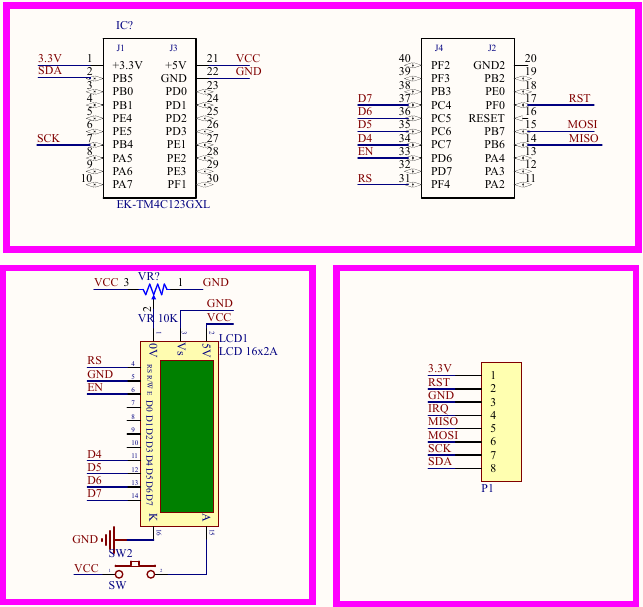
\includegraphics[scale=0.6]{images/schematic.png}
\caption{Schematic của hệ thống RFID}
\label{fig:schematic}
\end{figure}

\newpage
\subsection{Kết quả thực hiện PCB}
\subsubsection{Kết quả routing PCB}
\begin{figure}[ht]
\centering
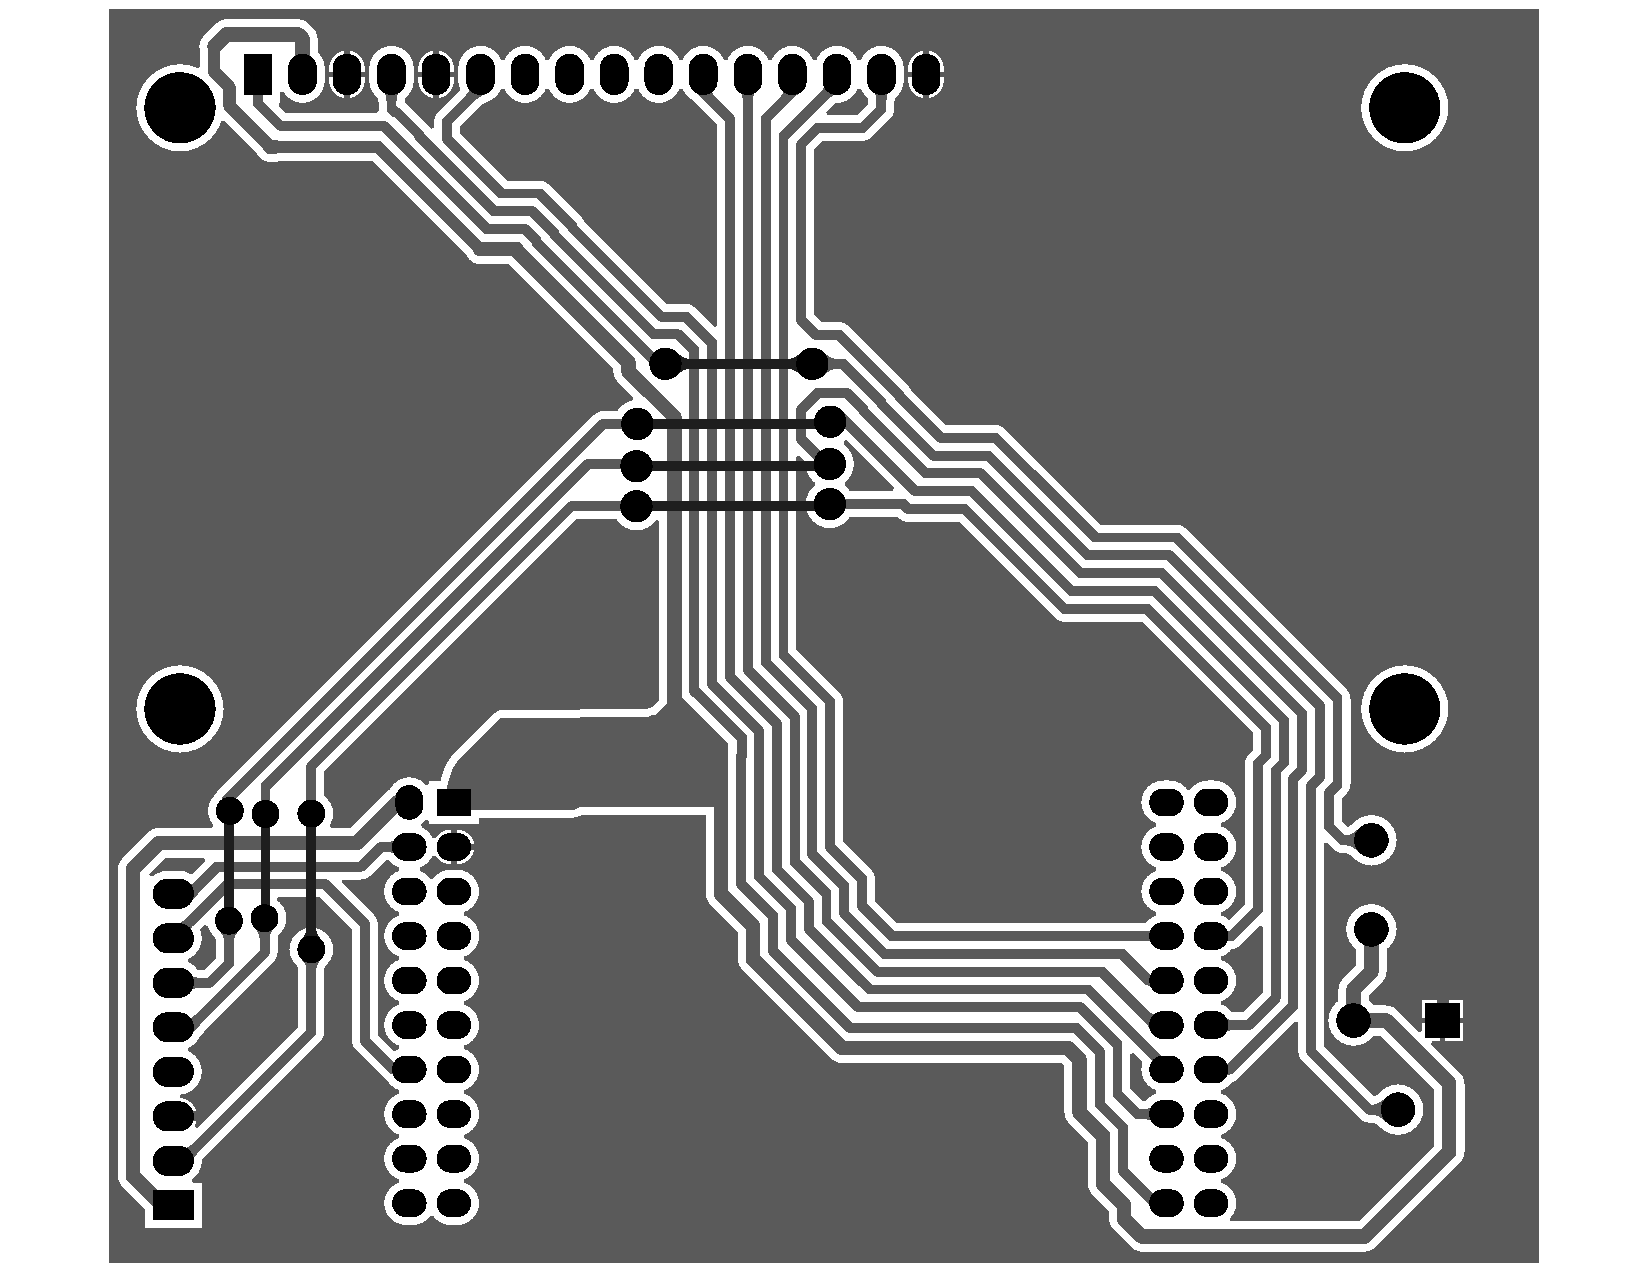
\includegraphics[scale=0.35]{images/routed.pdf}
\caption{Kết quả mạch sau khi thực hiện routing}
\end{figure}

\subsubsection{Kết quả mạch in}
\begin{figure}[ht]
\centering
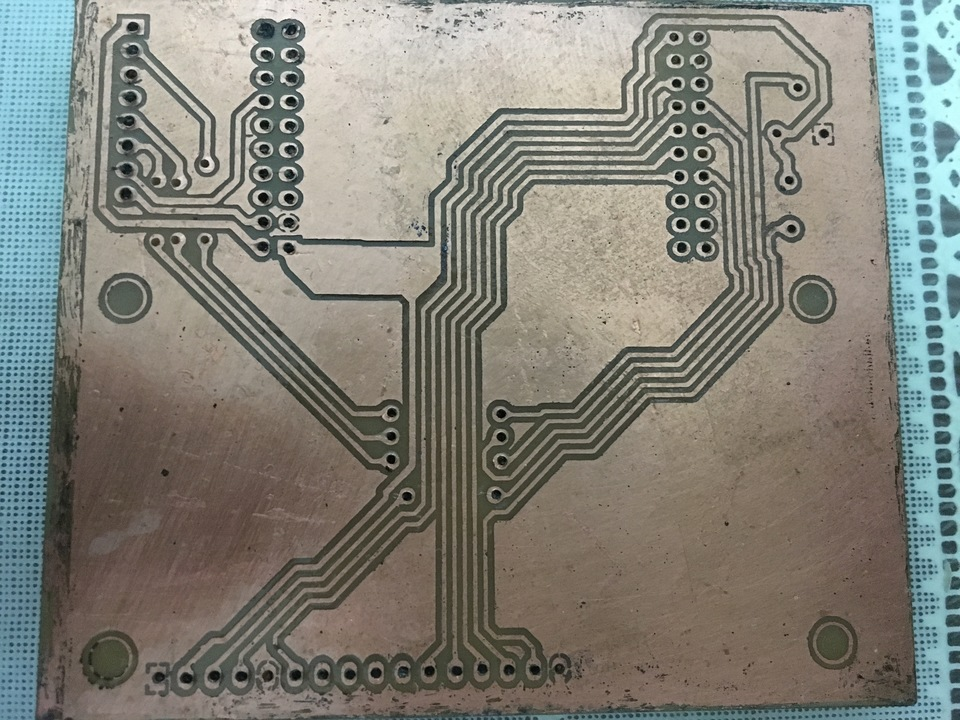
\includegraphics[scale=0.3]{images/board_output.jpg}
\caption{Kết quả mạch in}
\end{figure}

\newpage
\subsubsection{Kết quả mạch in đã gắn các linh kiện}
\begin{figure}[ht]
\centering
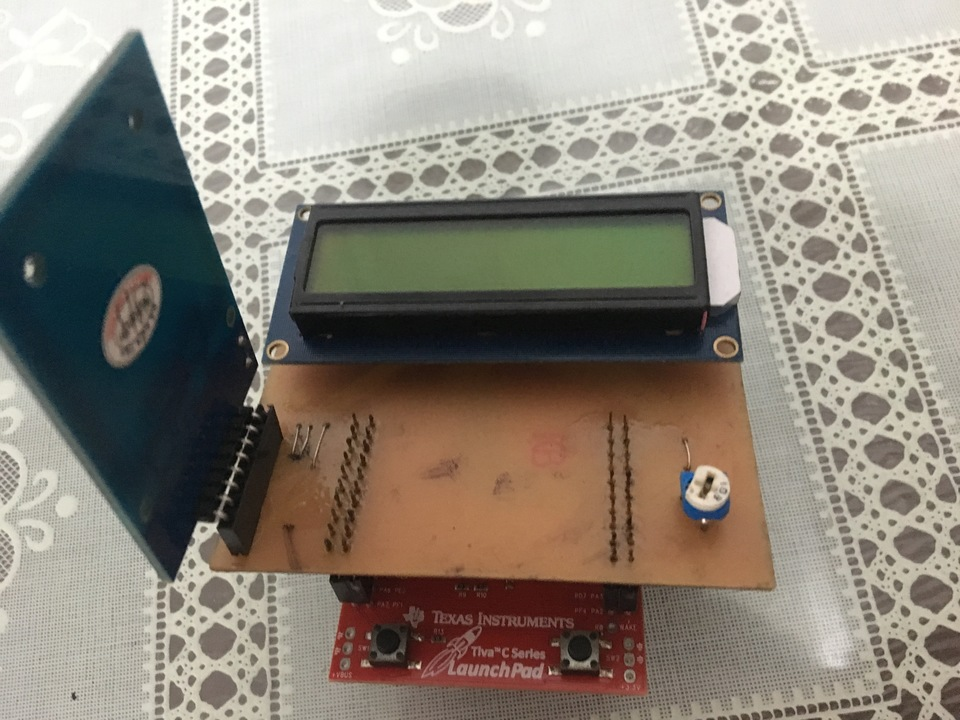
\includegraphics[scale=0.3]{images/board_finish.jpg}
\caption{Kết quả mạch in đã gắn các linh kiện}
\end{figure}

\section{Thực hiện phần mềm}
Source code của đề tài có thể xem tại phần phụ lục của bài báo cáo hoặc xem tại link: \url{https://github.com/Rudo2204/RC522-LCD-TM4C123G-CCS}.

Source code được chia làm 3 phần chính:
\begin{enumerate}
    \item Các file khởi chạy chương trình của đề tài được khởi tạo một cách tự động bởi phần mềm CCS.
        Nếu đề tài được phát triển sử dụng một phần mềm khác thì bỏ các file này.
    \item Thư mục \mintinline{bash}{LIB} chứa hai thư viện là thư viện module MFRC522 và thư viện LCD.

        - Thư viện module MFRC522 bao gồm các hàm khởi chạy và đọc/ghi thẻ,
        thư viện có nguồn gốc là từ thư viện MFRC522 của project Energia,
        nó đã được chỉnh sửa lại để có thể sử dụng trên phần mềm CCS và kit TIVA C trong đề tài này.

        - Thư viện LCD bao gồm các hàm khởi chạy và ghi vào LCD sử dụng GPIO trực tiếp.
        Nếu đề tài sử dụng các giao thức khác thì phải chỉnh sửa lại thư viện này.
    \item File \mintinline{bash}{main.c} là file chương trình chính của hệ thống,
        nó import nội dung từ thư viện \mintinline{bash}{TivaWare} từ bên ngoài và hai thư viện module MFRC522 và LCD trong source code của đề tài và thực hiện giải thuật của hệ thống (xem trang \pageref{ref:algorithm}).
\end{enumerate}

\chapter{Kết quả thực nghiệm}
\section{Cách thực hiện mô hình hệ thống}
Module MFRC522 khi mua ngoài thị trường có kèm theo hai tag như hình \ref{fig:default_tags}.
Ngoài ra, mô hình còn sử dụng một thẻ bên ngoài đó là thẻ sinh viên của Trường ĐH Bách Khoa
để chứng minh hệ thống có thể được áp dụng trong môi trường trường học thực tế.

Ở đây, tôi chọn mô phỏng mô hình điều khiển truy cập một cách đơn giản, lấy mã truy cập của tag xanh là tag gốc (master),
chỉ có tag xanh này mới có thể truy cập vào hệ thống, tất cả các tag còn lại đều sẽ bị từ chối.
Người dùng có thể dễ dàng thay đổi mã truy cập gốc này trong source code.
\begin{figure}[ht]
\centering
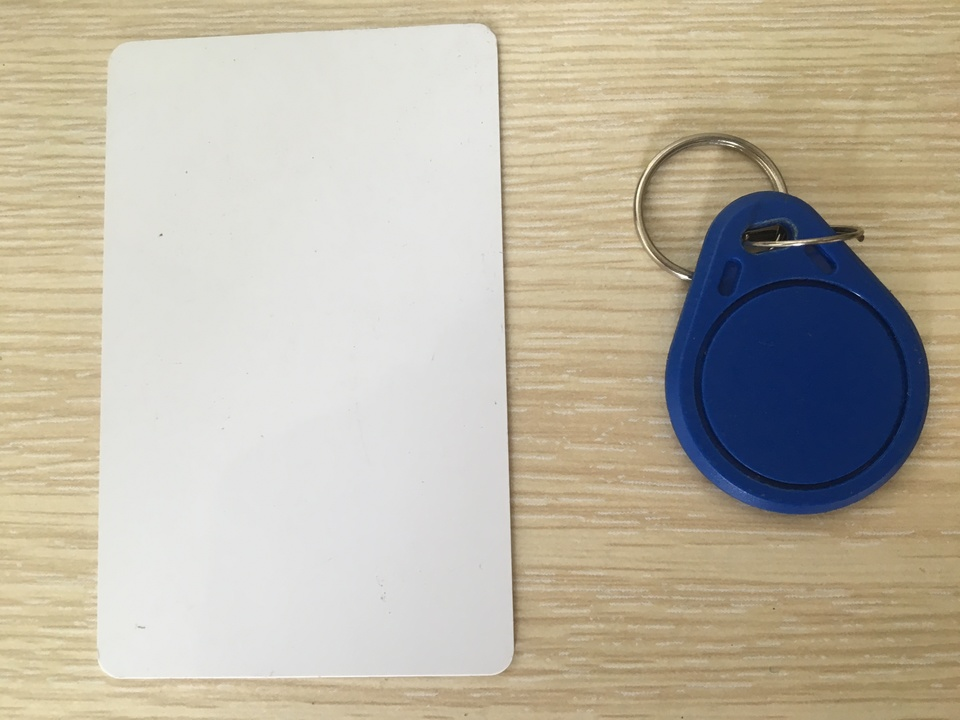
\includegraphics[scale=0.3]{images/default_tags.jpg}
\caption{Hai tag kèm theo module MFRC522}
\label{fig:default_tags}
\end{figure}

\section{Hình ảnh hệ thống khi chạy thực nghiệm}
\subsection{Hệ thống ở trạng thái mặc định}
Ở trạng thái mặc định, LCD hiển thị dòng chữ "Scan your card" báo hiệu hệ thống đang ở trang thái sẵn sàng đọc thẻ mới như ở hình \ref{fig:lcd_default}.
\begin{figure}[ht]
\centering
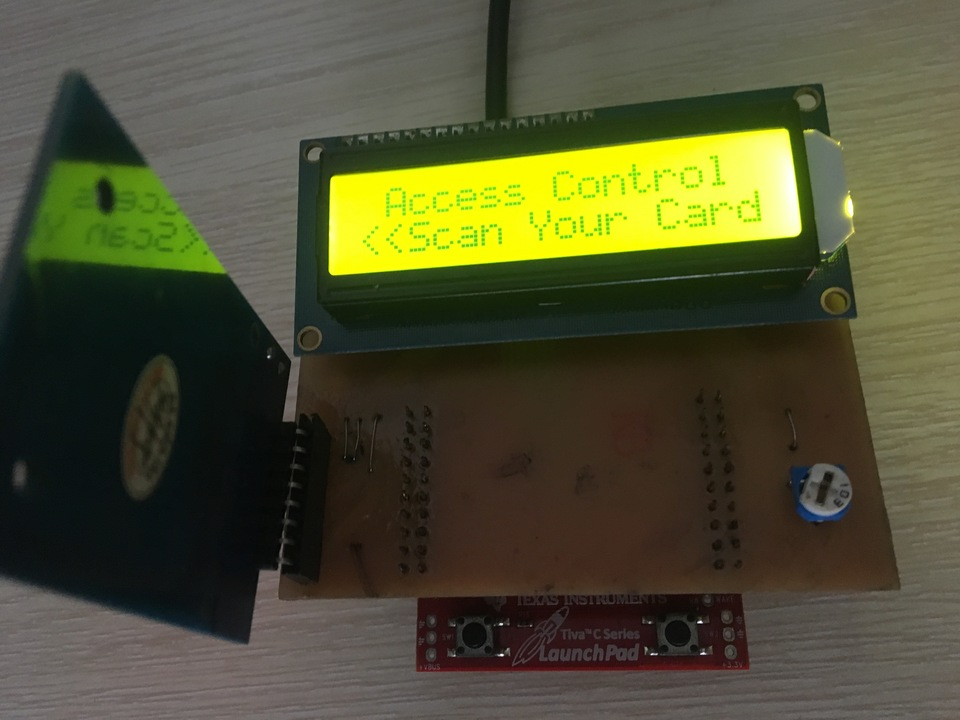
\includegraphics[scale=0.4]{images/lcd_default.jpg}
\caption{Hệ thống ở trạng thái mặc định}
\label{fig:lcd_default}
\end{figure}

Ngoài ra, sau khi hệ thống khởi động hoàn tất, hệ thống còn xuất ra một số thông tin của hệ thống qua UART.
Để bắt đầu nhận dữ liệu của hệ thống xuất qua UART đến máy tính chúng ta sử dụng lại thư viện \emph{serialport-rs}
bằng cách chạy phần mềm \emph{receive\_data} trên port kết nối với hệ thống sử dụng baud rate định sẵn trong source code
(ở đây là port \mintinline{bash}{/dev/ttyACM0} với baud rate 115200) với câu lệnh:\\
\mintinline{bash}{$ ./target/release/examples/receive_data /dev/ttyACM0 115200}

\newpage
Hình \ref{fig:UART_init_receive} mô tả cách thực hiện nhận dữ liệu qua UART trên máy tính.
Ở đây hệ thống xuất ra một số thông tin như giao tiếp đang được sử dụng, bit mode của SPI (ở đây là SPI 8-bit)
và phiên bản của module đọc thẻ và độ lợi của anten hệ thống (đơn vị là \si{decibel}).
\begin{figure}[ht]
\centering
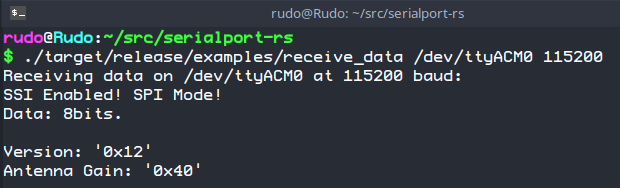
\includegraphics[scale=0.8]{images/UART_init_receive.png}
\caption{Các thông số ban đầu của hệ thống nhận qua UART}
\label{fig:UART_init_receive}
\end{figure}

\subsection{Thực hiện quét thẻ}
\subsubsection{Thực hiện quét tag master}
Thực hiện quét tag master vào hệ thống, hệ thống sẽ cho người dùng có tag master truy cập vào hệ thống (access granted) như hình \ref{fig:tag}.
\begin{figure}[ht]
\centering
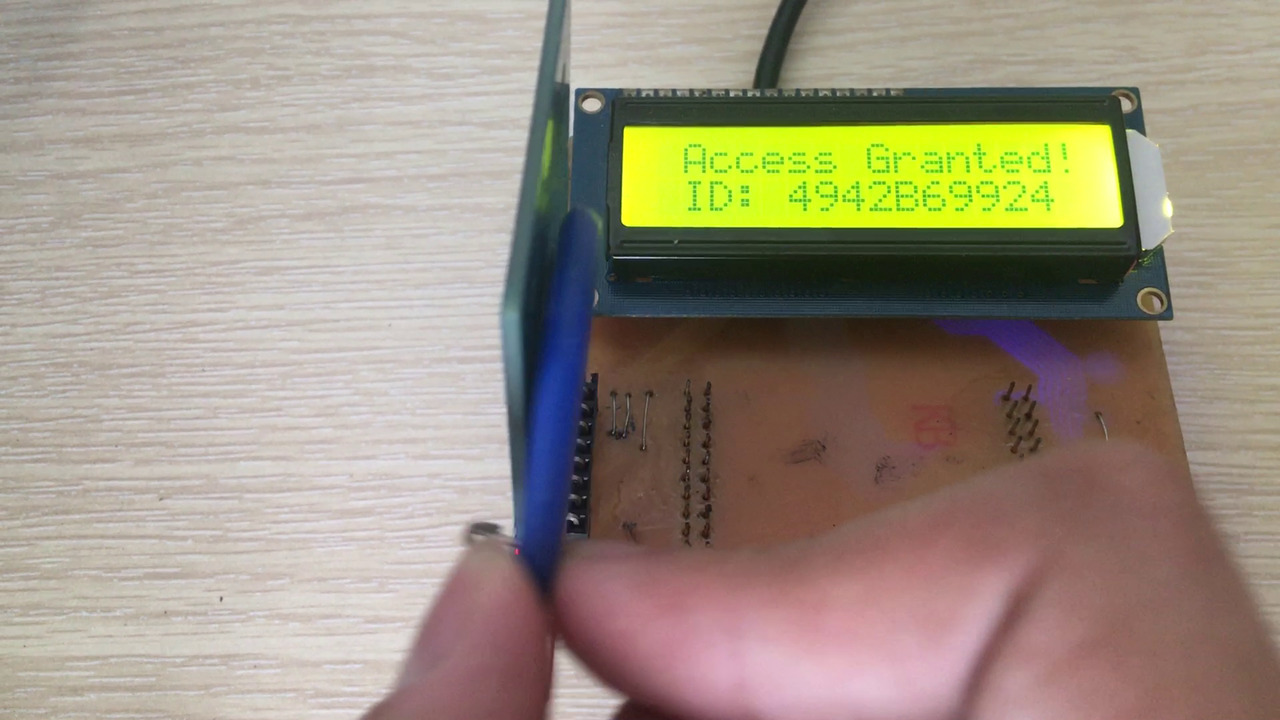
\includegraphics[scale=0.3]{images/tag.jpg}
\caption{Hệ thống cho phép truy cập với tag master}
\label{fig:tag}
\end{figure}

\newpage
\subsubsection{Thực hiện quét tag thường}
Thực hiện quét tag thường (ở đây là tag trắng) vào hệ thống, hệ thống từ chối truy cập vào hệ thống (access denied) như hình \ref{fig:card}.
\begin{figure}[ht]
\centering
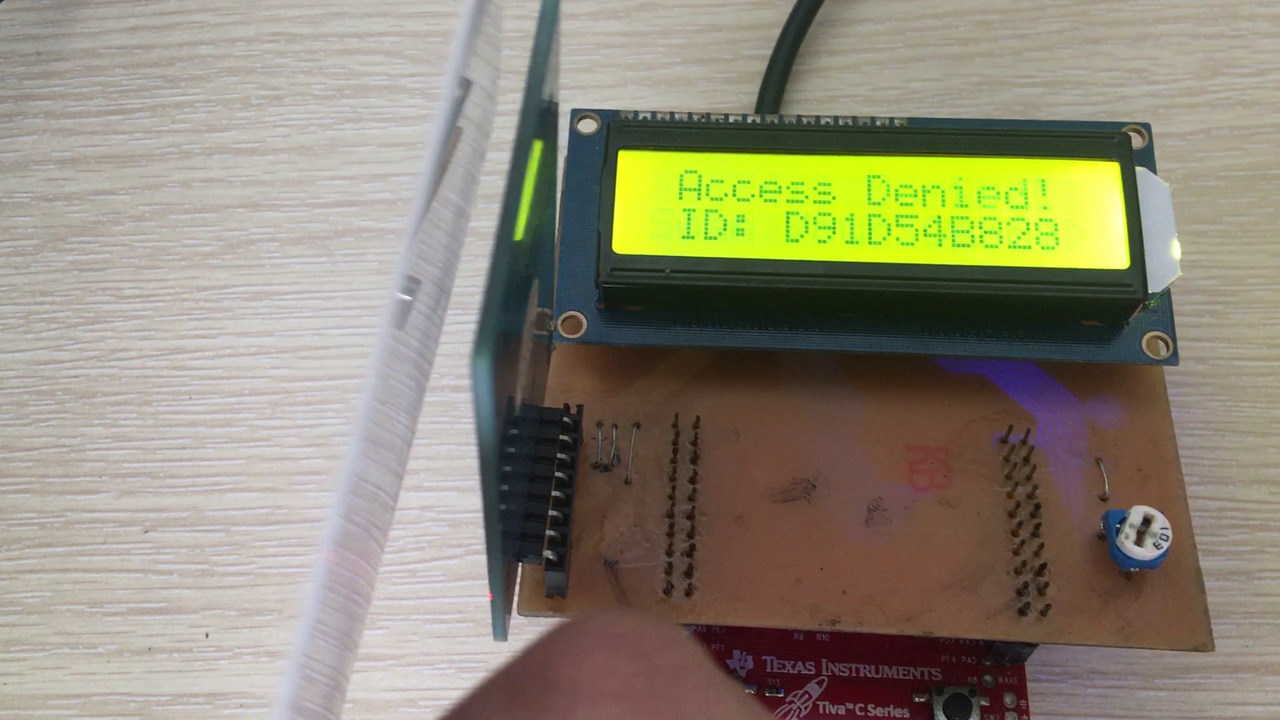
\includegraphics[scale=0.3]{images/card.jpg}
\caption{Hệ thống từ chối truy cập với tag thường}
\label{fig:card}
\end{figure}

\subsubsection{Thực hiện quét tag thường bên ngoài}
Thực hiện quét tag bên ngoài (ở đây là một thẻ sinh viên của Trường ĐH Bách Khoa) vào hệ thống, hệ thống từ chối truy cập vào hệ thống (access denied) như hình \ref{fig:student_card}.
\begin{figure}[ht]
\centering
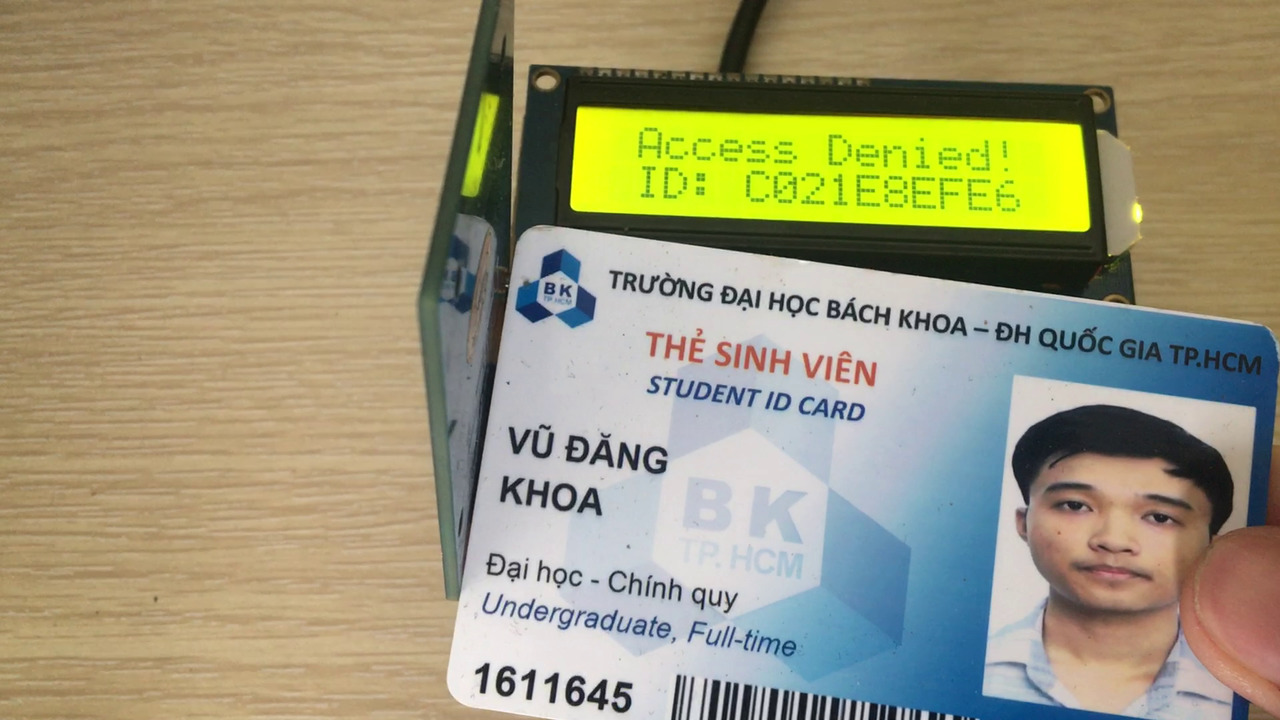
\includegraphics[scale=0.3]{images/student_card.jpg}
\caption{Hệ thống từ chối truy cập với tag thường bên ngoài}
\label{fig:student_card}
\end{figure}

\subsection{Dữ liệu các tag truyền qua UART}
Dữ liệu tag được quét cũng được truyền qua UART để người dùng có thể debug hoặc ứng dụng thêm các module khác để xử lý các dữ liệu này một cách tự động nhằm tăng hiệu quả của hệ thống nhận diện.

Hình \ref{fig:UART_data_receive} mô tả các dữ liệu các tag được quét truyền qua UART đến máy tính.
Ở đây, chỉ có dữ liệu UID của các tag được truyền qua UART, ngoài dữ liệu UID, ta còn có thể chỉnh sửa lại source code để lấy thêm các thông tin từ các data block của thẻ (nếu thẻ không bị mã hóa).
\begin{figure}[ht]
\centering
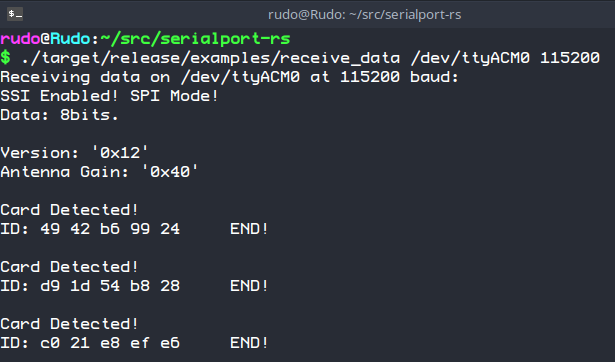
\includegraphics[scale=0.8]{images/UART_data_receive.png}
\caption{Dữ liệu tag được truyền qua UART}
\label{fig:UART_data_receive}
\end{figure}

\chapter{Kết luận và các hướng phát triển đề tài}
\section{Kết luận}
Đề tài này đã nêu ra lý thuyết và nêu ra một ứng dụng cụ thể của một hệ thống RFID trong môi trường thực tiễn.
Công nghệ RFID đã và đang mở ra một hướng mới cho vấn đề nhận diện mới, một hướng đã giải quyết được nhiều vấn đề đã bộc lộ trong các phương pháp nhận diện cũ,
tăng cao tính tiện lợi cho người dùng, nâng cao bảo mật và dễ dàng nâng cấp với hiệu quả cao với chi phí giá thành rẻ và thời gian thực hiện tương đối ngắn.
Trong tương lai gần, chắc chắn công nghệ RFID sẽ ngày càng được áp dụng rộng rãi hơn trong môi trường bệnh viện, trường học, công nghiệp, v.v..
\section{Các hướng phát triển đề tài}
Trong đề tài này, tôi mô phỏng một hệ thống nhận diện truy cập đơn giản.
Hệ thống này có thể được nâng cấp thành một ứng dụng thực tiễn bằng cách ứng dụng thêm một vài modules, ICs bên ngoài.

\textbf{Một vài ví dụ}:
\begin{itemize}
    \item Ứng dụng một module thẻ nhớ chứa cơ sở dữ liệu của các thẻ truy cập hệ thống, từ đó người dùng có thể cho phép các thẻ mới truy cập vào hệ thống trực tiếp mà không cần phải chỉnh sửa lại source code.
    \item Ứng dụng module kết nối internet: ứng dụng này tương tự như trên, hệ thống sẽ đọc dữ liệu từ internet và cho phép truy cập các thẻ mới hoặc từ chối truy cập cho các thẻ đã hết hạn/không còn hiệu lực.
    \item Ứng dụng thêm relay để tạo thành một hệ thống nhận dạng mở khóa cửa thông minh.
\end{itemize}
